%!TEX root = ../MasterThesis.tex

\section{System Design Proposal}
\label{sec:design_proposal}

As the previous section explained in detail, existing architectural approaches are of limited use for the design of a collaborative system to support the \gls{E-commerce} fraud investigation scenario described in Section~\ref{sec:scope_thesis}. The leading approach for such a system will have to combine the best properties from the Web Service and the Semantic Web designs. \\

As for the Web Service approach, the most valuable aspects of it are: \@

\begin{itemize}
	\item access to the \gls{HTTP} endpoint can be limited to a certain set of communication partners
	\item these partners have to authenticate with the Web Service first
	\item based on the identification of the partners only certain parts of information can be returned, and execution of operations can be restricted
\end{itemize}

Looking at the Semantic Web approach, it's most interesting functionalities are: \@

\begin{itemize}
	\item providing information in a semantically self-contained way
	\item the ability to merge information from different \gls{RDF} data stores
	\item the graph-based data model in \gls{RDF}
	\item the usage of \gls{SPARQL} to query the combined data set
\end{itemize}

In the following section the thesis will come up with an approach that uses the fundamental technologies from the Semantic Web for information sharing and integration as well as peer-to-peer communication technologies for securing and restricting access to the \gls{RDF} data sets from the relevant participants of the \gls{E-commerce} fraud investigation scenario. It will start with a discussion of the semantics of the underlying \gls{RDF} files and how these can be combined across various organizations. After that it shows how these information can be provided to the relevant parties in the investigation scenario. It will continue with a detailed look into the \gls{P2P} architectures that can be used for the proposed solution and will close with a conclusion about the solution that has been worked out.

\subsection{Vocabulary alignment}
\label{subsec:vocab_align}

The usage of the vocabulary of Schema.org is preferred as \ldots

\begin{figure}[H]
	\centering
		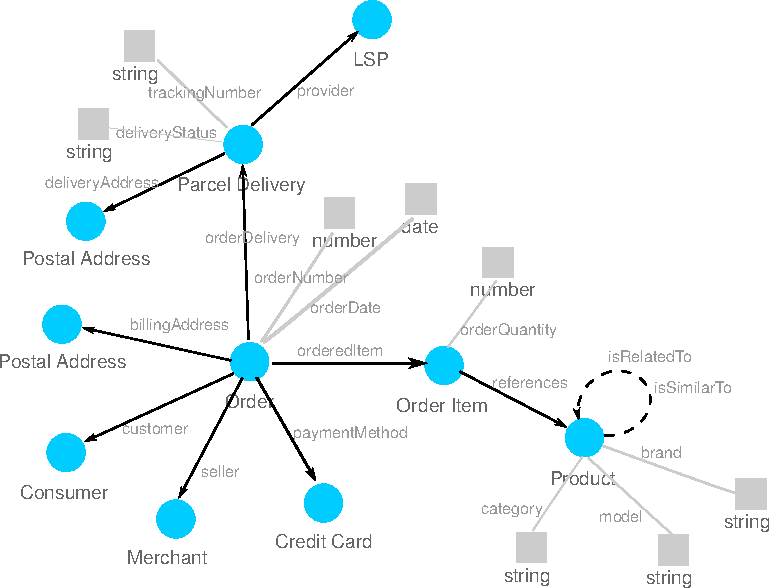
\includegraphics[width=0.8\columnwidth]{images/schema_org_mapping.pdf}
	\caption{Schema.org Mapping}
\label{fig:images_schema_org}
\end{figure}

% subsec vocab_align

\subsection{Communication protocols}
\label{subsec:comm_protocol}

As the merchants will provide semantic meta data for \gls{SEO} already, one can re-use part of these information for the E-commerce fraud investigation. The data is likely encoded in Microdata, \gls{RDFa} or \gls{JSON-LD}. \\

For the communication the \gls{WebRTC} is a good approach as it integrates well with existing enterprise IT infrastructures.

% subsec comm_protocol

\subsection{Partially centralized Peer-To-Peer System}
\label{subsec:p2p_partially_centralized_system}

The issuing bank is the trusted party in this system setup. It will initiate a data sharing session with the other required stakeholders based on the past usage of the credit card in question. During the P2P session the merchants, payment and logistic service providers will share the required information with the issuer. In this process the data from the other stakeholders will be replicated to the issuer, who will build up a graph based on the Schema.org schema mapping. The analysis of the data will be done on top of this graph by the issuer and can also be handled after the initial P2P data sharing session has been ended. If there are any new conclusions drawn from the data, the issuer is in charge to inform the stakeholders afterwards. So the main work will be on the issuer side, who is the major driving party in this scenario, as depicted in Figure~\ref{fig:images_p2p_centralized}.\@

\begin{figure}[H]
	\centering
		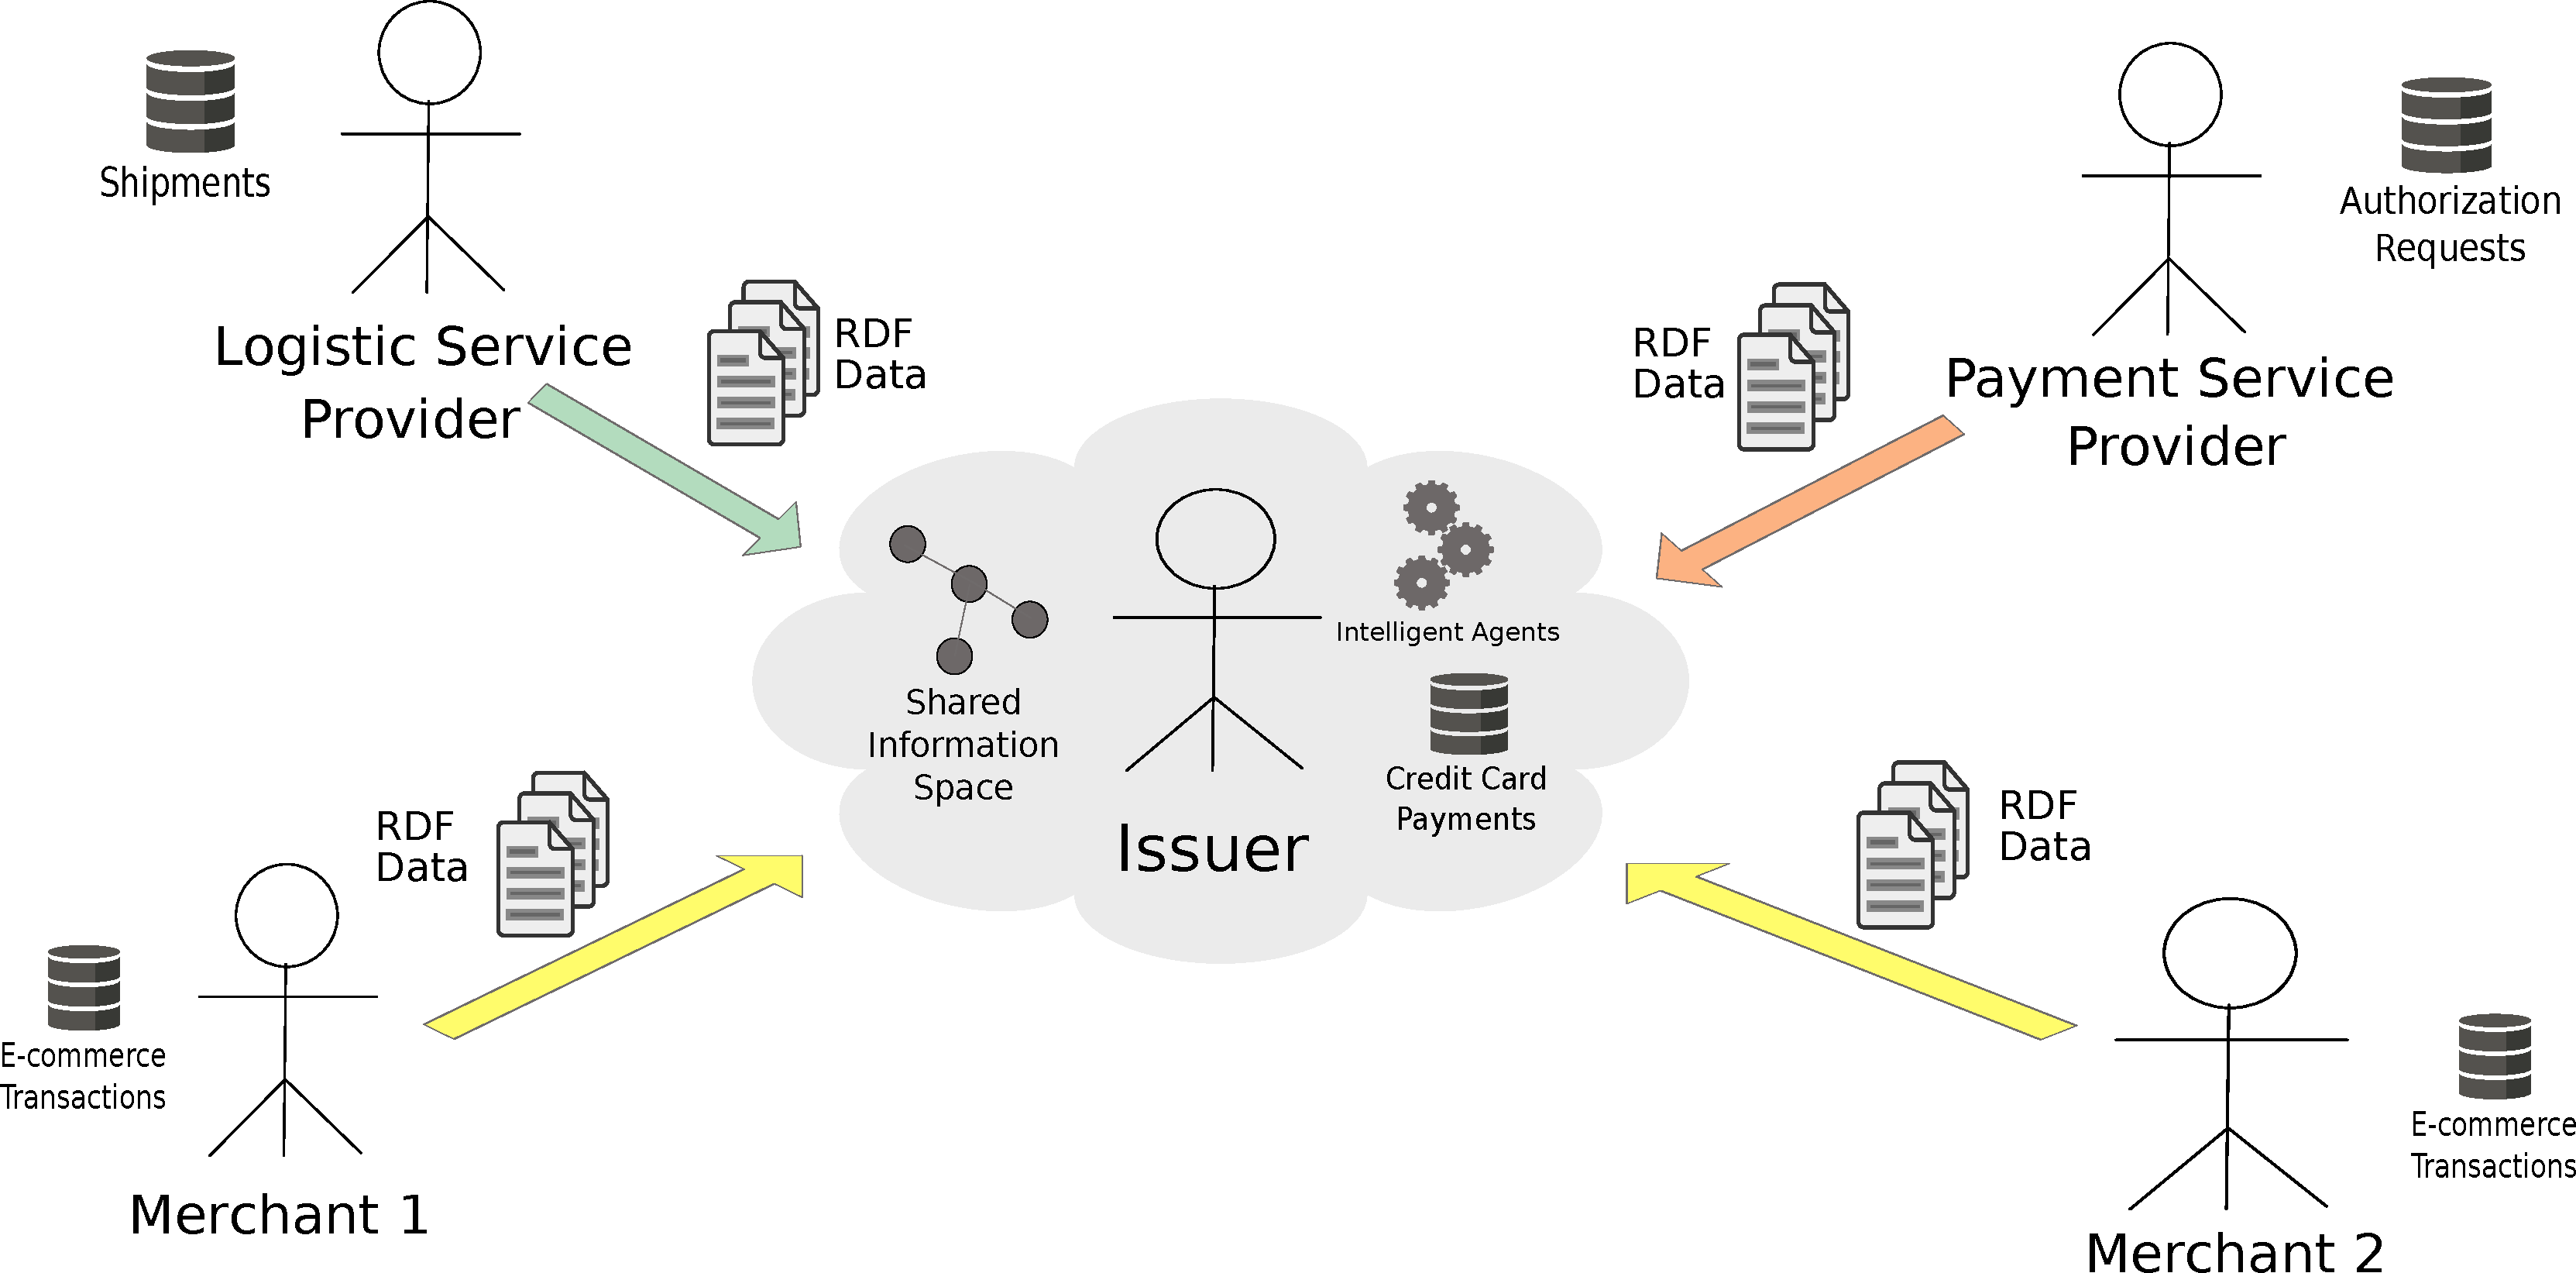
\includegraphics[width=0.8\columnwidth]{images/system_P2P_centralized.pdf}
	\caption{Partially centralized P2P system architecture}
\label{fig:images_p2p_centralized}
\end{figure}

Main issue with the above mentioned system architecture is, that the merchants, payment and logistic service providers have to hand over their information to the issuing bank of the credit card for analysis. This might be either problematic due to distrust of the objectives of the issuing bank, or not possible at all due to local data sharing restrictions and regulations.

% subsec p2p_partially_centralized_system

\subsection{Decentralized Peer-To-Peer System}
\label{subsec:p2p_decentralized_system}

In the decentralized P2P system architecture each node is equal and keeps their local data ready for analysis if the node is online. If the issuer will have to figure out, whether a transaction is fraudulent or not, she is going to send out various queries to all the available nodes in the P2P cluster asking for certain information that help investigating the case. The other nodes, whose reside on each stakeholder involved, will answering the queries based on the common Schema.org data mapping shown above and send back the results to the issuing bank. The issuer will collect all the results from the various parties and combine them to be able to analyze the issue and come up with a conclusion. The main benefit of this architecture is, that there is no need to duplicate the data from the other stakeholders to the issuing bank. Due to this it can also be a better suited solution if data sharing faces restrictions due to law or regulations. On the other hand this architecture will depend on the nodes being online all the time so the issuer can query for information at any time. So this works only in synchronous communication mode. Additionally there are efforts spread around all the stakeholders to set up and maintain a system for secure data querying functionality, please see Figure~\ref{fig:images_p2p_decentralized}.

\begin{figure}[H]
	\centering
		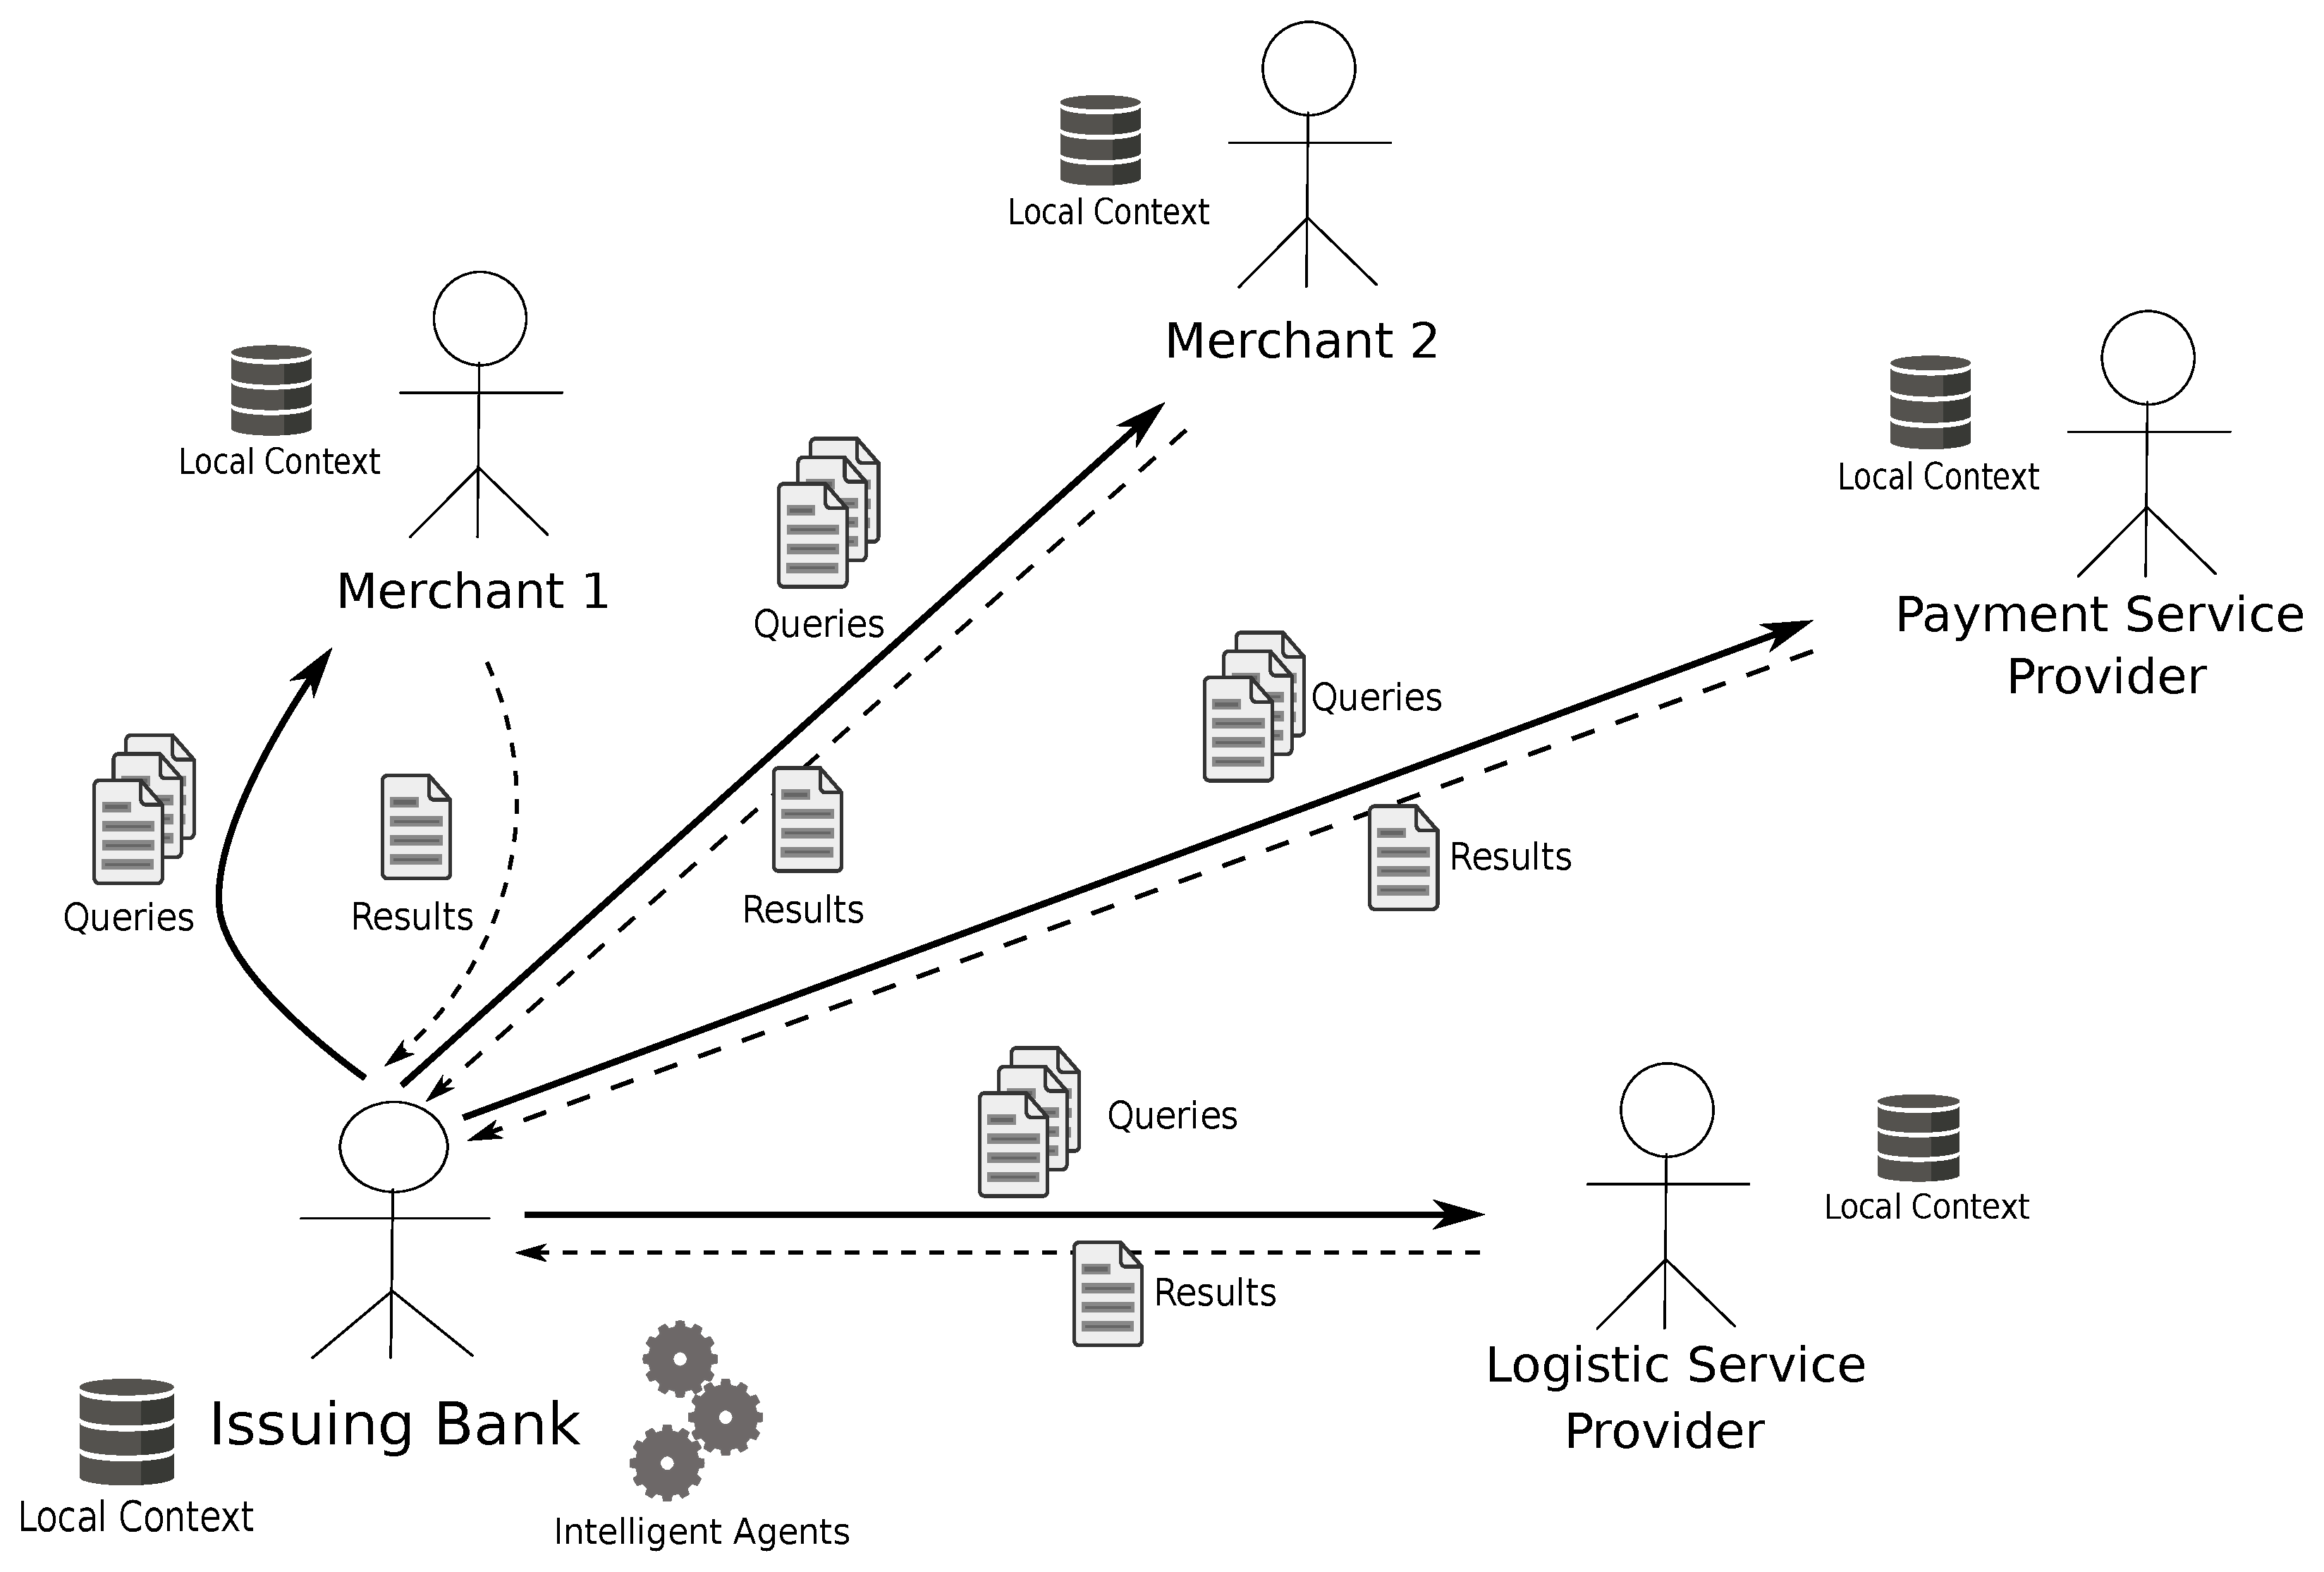
\includegraphics[width=0.8\columnwidth]{images/system_P2P_decentralized.pdf}
	\caption{Decentralized P2P system architecture}
\label{fig:images_p2p_decentralized}
\end{figure}

% subsec p2p_decentralized_system

\subsection{Proposed solution}
\label{subsec:proposed_solution}

% subsec proposed_solution

% section design_proposal (end)
